% ============================================================================
% DRAFT — Host/desktop phase (Windows) additions for main.tex
% Review, then integrate:
%   (A) Replace the current "Delivery channel: browser extension vs. desktop
%       client" subsection (main.tex ~L470) with, or follow it by, the
%       subsection below.
%   (B) Add \subsection{Action spectrum} to Results.
%   (C) Add the two limitation bullets to sec:limitations.
%   (D) Copy results/action_spectrum.pdf (or .png) into report/figures/ and
%       include the figure.
% Numbers are from data/raw/*/run_*.json and results/action-spectrum.md.
% ============================================================================

\subsection{Desktop and system-level exposure: an action spectrum}
\label{sec:action-spectrum}

To test whether the browser-extension finding generalises, we repeated the
measurement on the host operating system (Windows~11) against desktop
applications and the everyday act of \emph{opening} a received file. The same
synthetic document and planted secrets were used, captured with the same
\texttt{mitmproxy} add-on; interception on the host required trusting the proxy
CA in the Windows store and routing traffic through a system proxy that was
enabled only during capture. The results arrange themselves along a spectrum of
user action (Figure~\ref{fig:action-spectrum}).

\paragraph{Active submission leaks (as in the browser phase).} The
\textbf{DeepL} desktop client, given the document via paste for translation,
transmitted \textbf{100\%} of the characters and all twelve secrets --- including
the canary --- to \texttt{www2.deepl.com}. Notably the entire input was uploaded
even though the free tier only \emph{translated} the first 1500 characters: the
character cap is on the returned translation, not on what leaves the machine.

\paragraph{Passively opening a file usually leaks nothing.} Merely inserting a
USB stick containing the planted files caused no process to read their contents
(only the Windows Search indexer and shell hardware-detection probed volume
metadata and AutoPlay markers, per Process Monitor); nothing was transmitted.
Opening the plain-text file in Notepad, the PDF in Adobe Acrobat, the PDF in
Chrome (a browser laden with AI extensions), and the PDF in the Comet AI browser
each transmitted \textbf{0\%} of the document and \textbf{0/12} secrets. Two
mechanisms explain the browser negatives: Chrome renders local PDFs in a
sandboxed viewer that page-reading extensions cannot access without explicit
file-URL permission, and the Comet assistant does not scrape a tab's contents
until the user actively invokes it. Acrobat did contact Adobe's cloud on open
(telemetry and Document-Cloud UI), but transmitted none of the document's
contents in cleartext.

\paragraph{The exception: opening a document in Word.} Opening the same document
as a \texttt{.docx} in Microsoft~Word --- with no paste, no submission, nothing
but opening and reading it --- streamed \textbf{96.8\%} of the document, again
including every secret and the canary, to \texttt{augloop.svc.cloud.microsoft}
over a WebSocket. This host is Microsoft's ``Augmentation Loop,'' the cloud
backend for Office's Editor and Copilot intelligent services (the capture shows
posts to an \texttt{OfficeCopilotOrchestrationWorkflow}); these features are
enabled by default in Microsoft~365. Crucially the exfiltration came from the
\emph{default productivity suite itself}, not a third-party add-in: Grammarly,
though installed and running, sent only telemetry. This was captured over fully
decrypted HTTPS with zero TLS-handshake failures, i.e.\ high confidence.

\paragraph{Interpretation.} Exposure is \emph{surface-dependent}. Passively
receiving or opening a confidential file transmits nothing \emph{unless} the
application viewing it has a default cloud-AI integration watching the content.
Plain viewers (Notepad, Acrobat's local render, the browser PDF viewer) do not;
Word does. Combined with the browser phase and DeepL, the rule is: content
leaves the machine whenever it enters a surface an LLM-integrated service
monitors --- whether the user pastes it into a writing assistant or simply opens
it in a cloud-AI-enabled editor.

\begin{figure}[t]
  \centering
  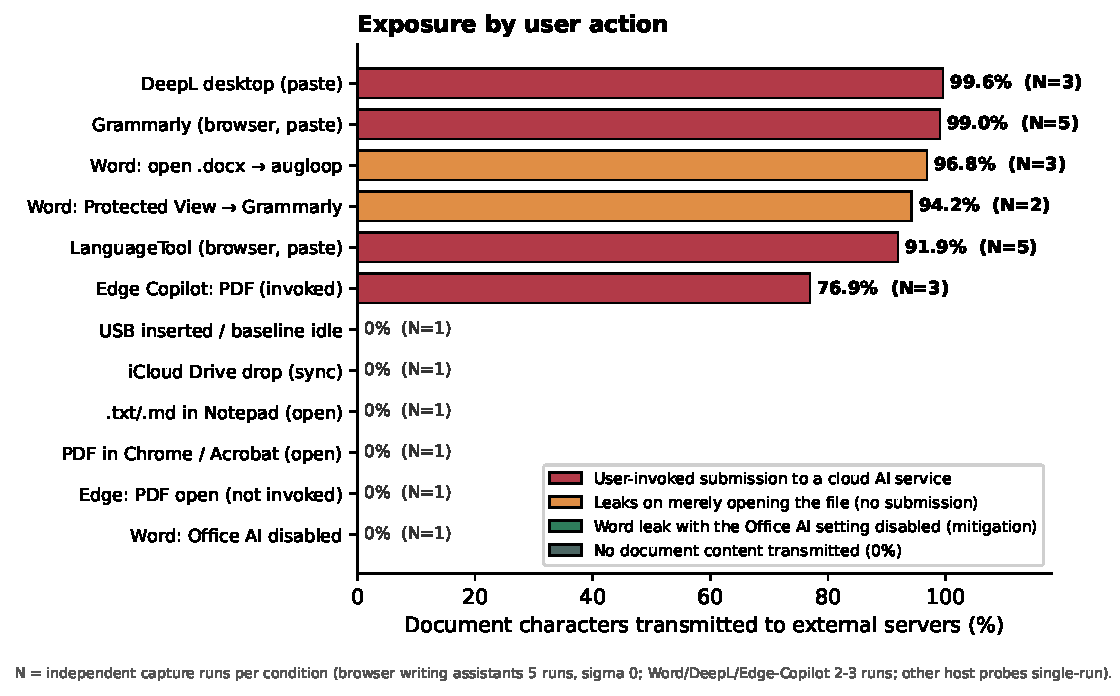
\includegraphics[width=\columnwidth]{figures/action_spectrum.pdf}
  \caption{Document characters transmitted to external servers, by user action.
  Active submission to an LLM tool (Grammarly, LanguageTool, DeepL) and
  \emph{opening} a document in Microsoft~Word leak nearly the entire document and
  every planted secret; passively inserting or opening the file in a non-AI
  viewer leaks nothing.}
  \label{fig:action-spectrum}
\end{figure}

% --- Additions for \section{Limitations and Excluded Tools} ---
% \paragraph{Host phase caveats.}
% \begin{itemize}[nosep]
%   \item \textbf{Certificate pinning (lower bound).} Several native Windows/
%         vendor channels (e.g.\ \texttt{*.events.data.microsoft.com}, some Adobe
%         and Google endpoints) refused interception, so their payloads are
%         opaque. Reported host-phase exposure is therefore a lower bound: we
%         count only what was decryptable.
%   \item \textbf{Single machine and configuration.} Host runs were on one
%         Windows~11 laptop signed into one Microsoft~365 account with Office AI
%         features at their defaults; the USB medium was a card-reader drive. The
%         Word/Office result is contingent on that default-on configuration and
%         would not occur with intelligent services disabled or an offline
%         account.
% \end{itemize}
